\section{HMM-DNN ASR}

\begin{frame}[plain]
  \centering
  \vspace{0.10\textheight}
  {\LARGE \textbf{Hybrid HMM-DNN ASR}}
  
  \vspace{0.08\textheight}
  {\large Transition to deep learning in acoustic modeling:\\Hybrid HMM-DNN systems}
\end{frame}


\begin{frame}{Objective function for DNN training: per-frame classification}
  \begin{itemize}
    \item \textbf{Supervised learning}, minimize our classification errors
    \item \textbf{Standard choice: Cross entropy loss function}
      \begin{itemize}
        \item Straightforward extension of logistic loss for binary
      \end{itemize}
  \end{itemize}
  \[
    Loss(x, y; W, b) = -\sum_{k=1}^{K} (y = k) \log f(x)_k
  \]
  \begin{itemize}
    \item This is a \textbf{frame-wise} loss. We use a label for each frame from a forced alignment
    \item Other loss functions possible. Can get deeper integration with the HMM or word error rate
  \end{itemize}
\end{frame}

% --- Stanford CS224S lec10, slides 10--14: neural acoustic modeling ---
\begin{frame}{Neural nets for acoustic modeling goes back to early speech}
  \centering
  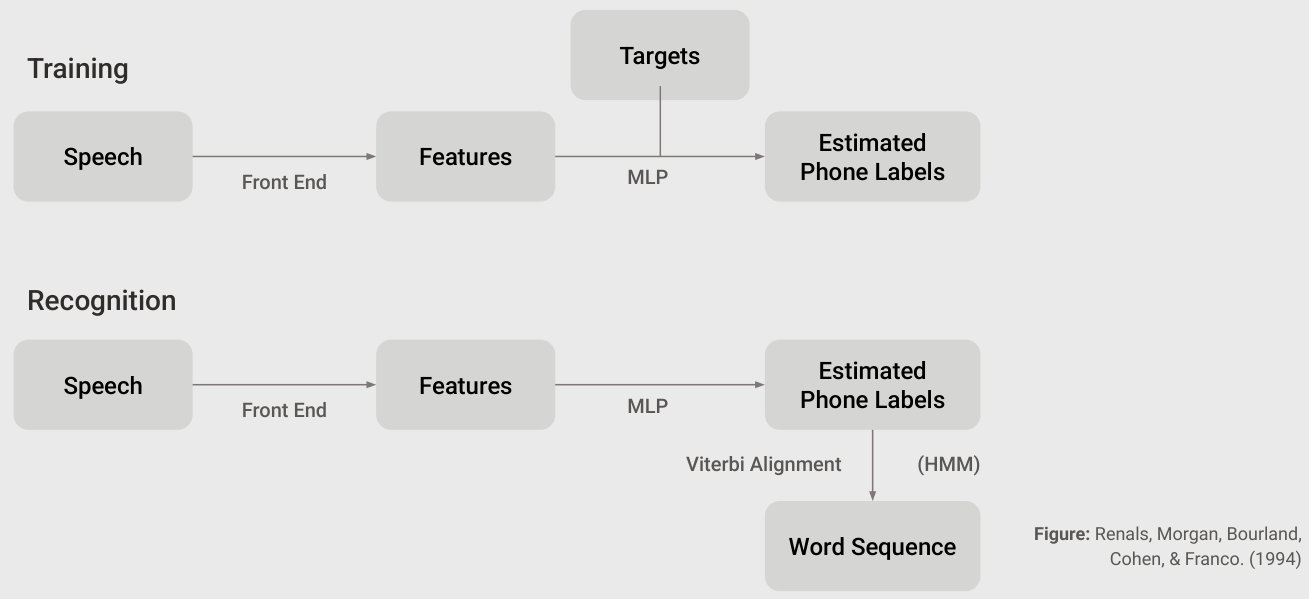
\includegraphics[width=\textwidth,height=0.78\textheight,keepaspectratio]{assets/New-Lecture-STT/cs224s_lec10_slide_10.png}
\end{frame}

\begin{frame}
  \frametitle{Early neural network approaches}
  \large
  \textit{Speech tasks motivated some of the original backpropagation work}
  \centering
  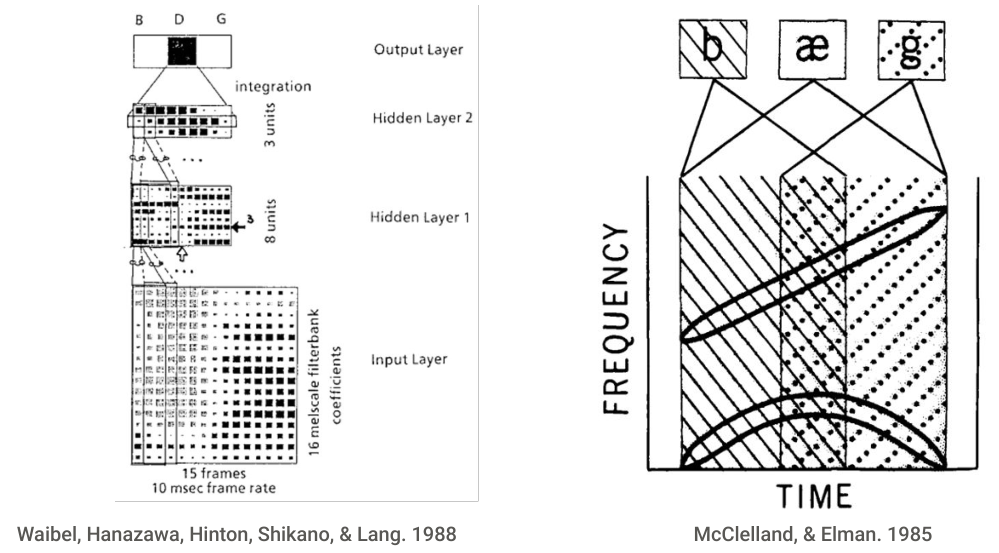
\includegraphics[width=\textwidth,height=0.78\textheight,keepaspectratio]{assets/New-Lecture-STT/cs224s_lec10_slide_11.png}
\end{frame}

\begin{frame}{Hybrid systems took over ASR around 2012-2015}
  \begin{itemize}
    \item DNN--HMM hybrids (Hinton et al., 2012) rapidly replaced GMM--HMM on large-vocabulary tasks.
    \item Sets the stage for deeper encoders, sequence training, and later end-to-end models.
  \end{itemize}
  \centering
  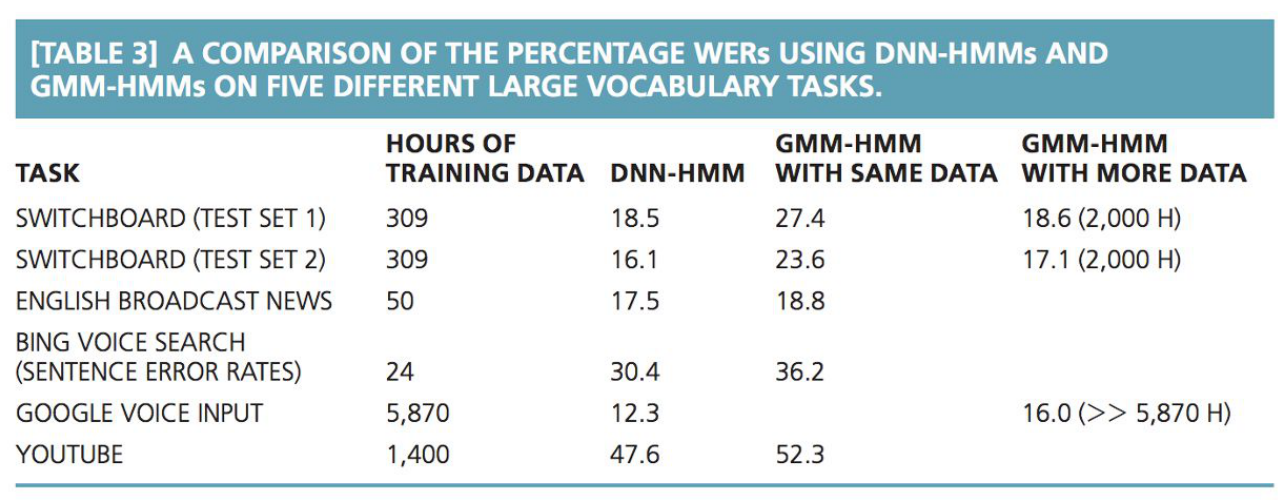
\includegraphics[width=\textwidth,height=0.72\textheight,keepaspectratio]{assets/New-Lecture-STT/cs224s_lec10_slide_13.png}
\end{frame}

\begin{frame}{What’s made modern DNNs successful?}
  \begin{itemize}
    \item Context-dependent HMM states
    \item Deeper nets improve on single hidden layer nets
    \item Hidden unit nonlinearity
    \item Many more model parameters (scaling up) \& large datasets
    \item Specific depth (e.g.\ 3 vs 7 hidden layers)
    \item Fast computers = run many experiments
    \item Architecture choices (easiest is replacing sigmoid)
    \item Pre-training \textcolor{red}{does not matter}*
    \begin{itemize}
      \item \textcolor{red}{Initially we thought this was the new trick that made things work}
    \end{itemize}
  \end{itemize}
\end{frame}

\begin{frame}{Recurrent DNN hybrid acoustic models}
  \centering
  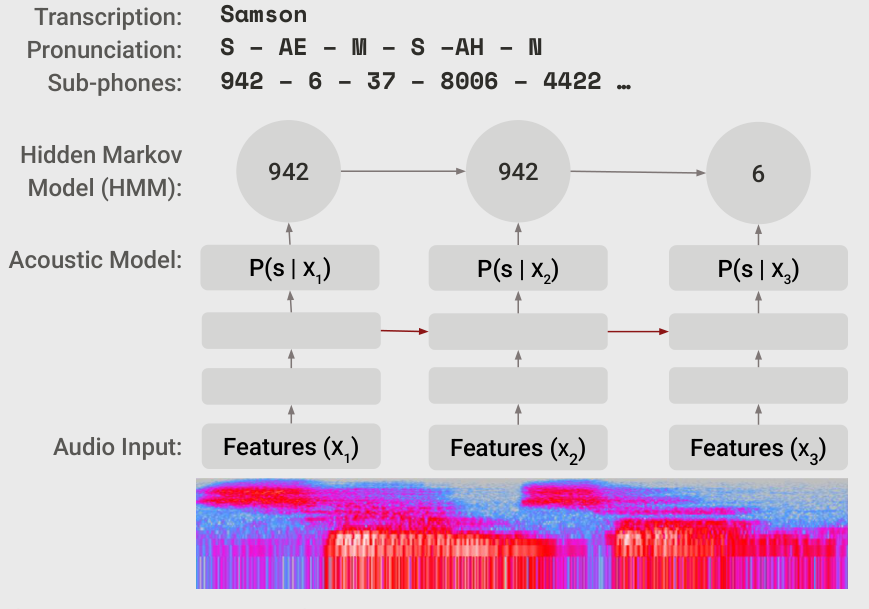
\includegraphics[width=\textwidth,height=0.92\textheight,keepaspectratio]{assets/New-Lecture-STT/cs224s_lec10_slide_15.png}
\end{frame}

\begin{frame}{Deep recurrent networks}
  \centering
  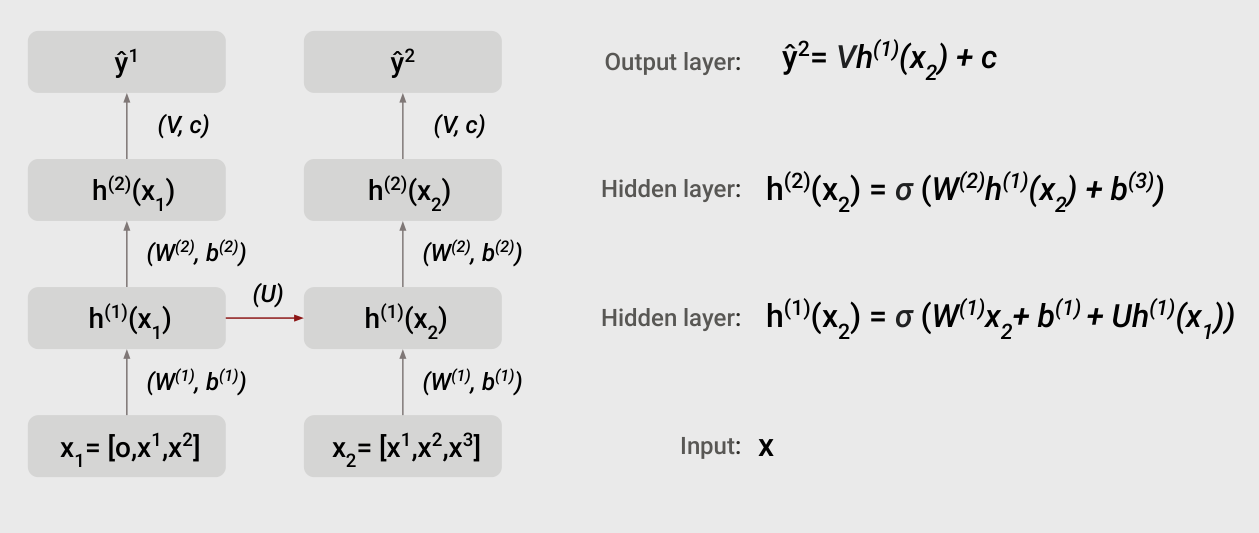
\includegraphics[width=\textwidth,height=0.92\textheight,keepaspectratio]{assets/New-Lecture-STT/cs224s_lec10_slide_16.png}
\end{frame}

\begin{frame}{How can we improve upon HMM-DNN?}
  \begin{itemize}
    \item Lexicon introduces too many pronunciation assumptions. Requires hand engineering.
    \item Iteratively building HMM systems requires complex ``recipes'' to progressively improve alignments + acoustic models.
    \item HMM-DNN systems perform better, but still require the above
    \begin{itemize}
      \item Can we use deep learning approaches to replace the HMM-based approaches so far?
    \end{itemize}
  \end{itemize}
  \vspace{1em}
\end{frame}
